%%%%%%%%%%%%%%%%%%%%%%%%%%%%%%%%%%%%%%%%%%%%%%%%%%%%%%%%%%%%%%%%%%%%%%%%%%%%%%
%  FairML Project — Study Guide
%  A ground-up explanation of the project: overview, terms, metrics,
%  methodology, results, and paper preparation. With worked examples.
%
%  COMPILE: pdfLaTeX  (guide.tex)
%%%%%%%%%%%%%%%%%%%%%%%%%%%%%%%%%%%%%%%%%%%%%%%%%%%%%%%%%%%%%%%%%%%%%%%%%%%%%%
\documentclass[11pt,a4paper]{article}

\usepackage[T1]{fontenc}
\usepackage[utf8]{inputenc}
\usepackage{lmodern}
\usepackage{microtype}
\usepackage[margin=1in,headheight=14pt]{geometry}
\usepackage{amsmath,amssymb}
\usepackage{graphicx}
\graphicspath{{figures/}}
\usepackage{booktabs}
\usepackage{longtable}
\usepackage{array}
\usepackage{multirow}
\usepackage[table,dvipsnames]{xcolor}
\usepackage{tcolorbox}
\tcbuselibrary{skins,breakable}
\usepackage{enumitem}
\usepackage{fancyhdr}
\usepackage{titlesec}
\usepackage{tikz}
\usetikzlibrary{shapes.geometric,arrows.meta,positioning,calc}
\usepackage[htt]{hyphenat}
\usepackage[hidelinks]{hyperref}
\emergencystretch=3em
\hbadness=2000

% ---- palette -----------------------------------------------------------------
\definecolor{ink}{HTML}{1F2933}
\definecolor{accent}{HTML}{1F6F8B}
\definecolor{accentlt}{HTML}{E8F1F4}
\definecolor{warn}{HTML}{B45309}
\definecolor{warnlt}{HTML}{FDF3E3}
\definecolor{good}{HTML}{2F7A4E}
\definecolor{goodlt}{HTML}{EAF4EE}
\definecolor{rule}{HTML}{C9D3D9}

\color{ink}

% ---- headings ----------------------------------------------------------------
\titleformat{\section}{\Large\bfseries\color{accent}}{\thesection}{0.7em}{}
\titleformat{\subsection}{\large\bfseries\color{ink}}{\thesubsection}{0.6em}{}
\titleformat{\subsubsection}{\normalsize\bfseries\color{ink}}{\thesubsubsection}{0.5em}{}
\titlespacing*{\section}{0pt}{2.2ex plus 1ex minus .2ex}{1.2ex plus .2ex}

\pagestyle{fancy}\fancyhf{}
\renewcommand{\headrulewidth}{0.4pt}
\fancyhead[L]{\small\color{accent}FairML — Project Study Guide}
\fancyhead[R]{\small\thepage}

% ---- boxes -------------------------------------------------------------------
\newtcolorbox[auto counter,number within=section]{example}[1][]{
  breakable, enhanced, colback=accentlt, colframe=accent,
  boxrule=0.5pt, left=8pt, right=8pt, top=6pt, bottom=6pt, arc=2pt,
  fonttitle=\bfseries\small, coltitle=white,
  title={Worked Example~\thetcbcounter\ifx\relax#1\relax\else: #1\fi}}

\newtcolorbox{warnbox}[1][]{
  breakable, enhanced, colback=warnlt, colframe=warn,
  boxrule=0.5pt, left=8pt, right=8pt, top=6pt, bottom=6pt, arc=2pt,
  fonttitle=\bfseries\small, coltitle=white,
  title={\ifx\relax#1\relax Caution\else#1\fi}}

\newtcolorbox{keybox}[1][]{
  breakable, enhanced, colback=goodlt, colframe=good,
  boxrule=0.5pt, left=8pt, right=8pt, top=6pt, bottom=6pt, arc=2pt,
  fonttitle=\bfseries\small, coltitle=white,
  title={\ifx\relax#1\relax Key Idea\else#1\fi}}

\newcommand{\dpdtwo}{\ensuremath{\mathrm{DPD}_{2}}}
\newcommand{\getwo}{\ensuremath{\mathrm{GE}(2)}}
\newcommand{\code}[1]{\texttt{\small #1}}
\newcommand{\file}[1]{\textcolor{accent}{\texttt{\small #1}}}

\newcolumntype{L}[1]{>{\raggedright\arraybackslash}p{#1}}
\setlist[itemize]{leftmargin=1.3em,itemsep=2pt,topsep=3pt}
\setlist[enumerate]{leftmargin=1.5em,itemsep=2pt,topsep=3pt}

\begin{document}
\sloppy

%%%%%%%%%%%%%%%%%%%%%%%%%%%%%%%%%%%%%%%%%%%%%%%%%%%%%%%%%%%%%%%%%%%% TITLE PAGE
\begin{titlepage}
\centering
\vspace*{2.5cm}
{\Huge\bfseries\color{accent} FairML\par}
\vspace{0.5cm}
{\LARGE Project Study Guide\par}
\vspace{0.8cm}
{\large Understanding the group--individual fairness trade-off study\\
from first principles\par}
\vspace{1.4cm}
\rule{0.75\textwidth}{0.8pt}\par
\vspace{0.8cm}
\begin{minipage}{0.8\textwidth}
\centering\large
Overview \,\textbullet\, Terminology \,\textbullet\, Metrics \,\textbullet\,
Methodology \,\textbullet\, Results \,\textbullet\, Paper Preparation
\end{minipage}
\par\vspace{0.8cm}
\rule{0.75\textwidth}{0.8pt}\par
\vfill
\begin{minipage}{0.85\textwidth}
\small
\textbf{How to read this document.} Every section starts with a plain-language
explanation and then gives the technical version. Blue boxes are worked
numerical examples you can verify by hand. Amber boxes flag things that are
wrong, misleading, or easy to misread in the current project. Green boxes are
the ideas worth memorising.

\vspace{4pt}
\textbf{Everything here is grounded in the actual code and result files.}
Where a value has no accepted standard, this guide says so explicitly rather
than inventing a threshold.
\end{minipage}
\vfill
{\small Generated \today\par}
\end{titlepage}

\tableofcontents
\newpage

%%%%%%%%%%%%%%%%%%%%%%%%%%%%%%%%%%%%%%%%%%%%%%%%%%%%%%%%%% 1. PROJECT OVERVIEW
\section{Project Overview}

\subsection{What problem are we trying to solve?}

When a machine-learning model makes decisions about people --- will this
defendant re-offend? should this person get a loan? does this person earn more
than \$50{,}000? --- it can be unfair in \textbf{two different ways}, and
those two ways are not the same thing.

\begin{center}
\small
\begin{tabular}{@{}p{0.19\textwidth}p{0.35\textwidth}p{0.38\textwidth}@{}}
\toprule
\textbf{Kind of fairness} & \textbf{The question it asks} & \textbf{Example complaint} \\
\midrule
\textbf{Group fairness} &
Are demographic groups treated equally \emph{on average}? &
``Black defendants are flagged high-risk far more often than white defendants.'' \\
\addlinespace
\textbf{Individual fairness} &
Are the model's mistakes spread evenly across \emph{individuals}, or do a few
people absorb all the harm? &
``Overall the groups look balanced, but a small set of people get wrecked by
the errors.'' \\
\bottomrule
\end{tabular}
\end{center}

The uncomfortable part: \textbf{fixing one can break the other.} Forcing every
group to have the same approval rate means you must approve some people you
would otherwise reject, and reject some you would otherwise approve. Those
forced flips are extra errors, and they land on specific individuals.

There is a well-known body of theory saying certain fairness definitions are
mathematically incompatible. What is much thinner in the literature is
\textbf{empirical measurement}: if you actually build a model and turn a dial
from ``optimise group fairness'' toward ``optimise individual fairness,'' what
happens to each metric, on real data, with real error bars?

\subsection{What is the main objective?}

\begin{keybox}[The one-sentence framing]
The composite loss is the \textbf{instrument}; the trade-off map is the
\textbf{contribution}.
\end{keybox}

We are \emph{not} claiming ``we invented a better fairness algorithm.'' We are
claiming: ``we built a dial, turned it across three datasets $\times$ two model
types $\times$ ten random seeds, and here is the empirical map of what the
trade-off actually looks like.''

Three research questions drive everything:

\begin{description}[leftmargin=3.2em,style=nextline,font=\bfseries\color{accent}]
\item[RQ1] Is there a \emph{measurable} tension between group fairness
(DPD/EOD) and individual fairness (GE) when each is optimised directly?
\item[RQ2] Is the tension consistent across datasets (race/COMPAS, sex/German,
sex/Adult) and model classes (logistic regression, MLP)?
\item[RQ3] Where does our composite-loss frontier sit relative to established
pre-, in-, and post-processing fairness methods?
\end{description}

\subsection{Why does this problem matter?}

\begin{enumerate}
\item \textbf{Real deployments must pick one.} A bank or court system
implementing a ``fairness requirement'' has to choose a definition. If the
definitions trade off against each other, that choice has a real cost, and
practitioners deserve to know its size.
\item \textbf{Regulation is definition-blind.} Rules say ``don't
discriminate,'' not ``keep demographic parity difference below 0.05.''
Empirical trade-off maps are what translate a legal requirement into an
engineering target.
\item \textbf{Impossibility theorems say ``you can't have both,'' not ``how
much does each cost.''} Ours is a magnitude study.
\end{enumerate}

\subsection{What is the overall approach?}

Build a single loss function with two knobs.

\begin{itemize}
\item $\boldsymbol{\alpha}$ controls how much you care about \emph{accuracy
versus fairness at all}.
\item $\boldsymbol{\beta}$ controls, \emph{within} the fairness part, how much
is group fairness versus individual fairness.
\end{itemize}

Then sweep a $7\times7$ grid of $(\alpha,\beta)$, training a model at every
grid point, on three datasets, with two architectures, repeated over ten random
seeds --- about \textbf{2{,}940 trained models} --- and measure six metrics on
each. Compare against six established baselines. Test significance with a
paired non-parametric test across seeds.

%%%%%%%%%%%%%%%%%%%%%%%%%%%%%%%%%%%%%%%%%%%%%%%%%%%%%%%% 2. TERMS AND CONCEPTS
\section{Important Terms and Concepts}

\subsection{The basic setup}

\begin{description}[leftmargin=0em,style=nextline,itemsep=5pt]

\item[Binary classification]
The model outputs one number per person, and you threshold it at $0.5$ to get a
yes/no decision. All three datasets in this project are binary.

\item[Sensitive attribute (also: protected attribute)]
The demographic variable that fairness is measured \emph{with respect to}. In
this project: \code{race} on COMPAS, \code{Sex} on German, \code{sex} on Adult.

\item[Positive class]
The outcome coded as $1$. We deliberately made this the \emph{adverse} outcome
on COMPAS and German so the datasets align: COMPAS \code{two\_year\_recid} $=$
re-offended; German \code{risk} $=1$ means \textbf{bad} credit. Adult breaks the
pattern --- there $1 =$ income $>$ \$50K, a \emph{good} outcome.

\item[Logit]
The raw pre-sigmoid score. Our models return logits; the sigmoid is applied
inside the loss. (This fixed a double-sigmoid bug in the legacy code.)

\item[Sigmoid]
Squashes a logit into a probability: $\sigma(z) = 1/(1+e^{-z})$.

\item[BCE (Binary Cross-Entropy)]
The standard accuracy loss for binary classification. Penalises confident wrong
answers heavily.

\end{description}

\begin{warnbox}[Design choice reviewers will ask about]
The sensitive attribute is \textbf{left in the feature matrix} and fed to the
model. This is a legitimate choice (``fairness through awareness'' --- hiding
the attribute doesn't help because proxies exist), but state it deliberately in
the paper rather than leaving it implicit.
\end{warnbox}

\subsection{The models}

\begin{description}[leftmargin=0em,style=nextline,itemsep=5pt]
\item[Logistic Regression (LR)]
One linear layer, one output. Simple, interpretable, the field-standard
fairness baseline.

\item[MLP (Multi-Layer Perceptron), 64--64]
Input $\to$ 64 $\to$ ReLU $\to$ 64 $\to$ ReLU $\to$ 1. A small neural network.
Its role is to answer RQ2's ``does this hold for a nonlinear model too?''

\item[ReLU] Activation function, $\max(0,x)$, gives the network nonlinearity.

\item[Adam] The optimiser. Learning rate $0.01$, weight decay $10^{-4}$.

\item[Weight decay (L2 regularisation)]
Shrinks weights toward zero to prevent overfitting.

\item[Early stopping]
Stop training when validation loss stops improving. Patience $=20$ epochs, and
it \emph{deep-copies} the best weights rather than holding a live reference ---
that was a real bug in the legacy code.
\end{description}

\begin{warnbox}[Training detail worth stating explicitly]
The training loop does \textbf{one optimiser step per epoch on the full
dataset} --- full-batch gradient descent, not mini-batch SGD. With
\code{num\_epochs=300} that is at most 300 gradient steps. This is a deliberate
consequence of the loss design (SoftDP needs all groups present in the batch to
compute a group gap), and it is fine for tabular data of this size. But say it
explicitly --- reviewers will otherwise assume mini-batching.
\end{warnbox}

\subsection{The knobs: \texorpdfstring{$\alpha$}{alpha} and
\texorpdfstring{$\beta$}{beta}}

The whole project lives in this equation:
\begin{equation}
\mathcal{L} \;=\; \alpha \cdot \mathrm{BCE}
\;+\; (1-\alpha)\Big[\,\beta \cdot \mathrm{SoftDP} \;+\; (1-\beta)\cdot \mathrm{SoftGE}\,\Big]
\label{eq:composite}
\end{equation}

\begin{center}
\small
\begin{tabular}{@{}llp{0.52\textwidth}@{}}
\toprule
\textbf{Knob} & \textbf{Value} & \textbf{Meaning} \\
\midrule
\multirow{3}{*}{$\alpha$}
 & $1$   & Pure BCE, no fairness term at all. This is the \textbf{baseline}. \\
 & $0$   & Fairness only, accuracy ignored $\to$ degenerate models. \\
 & swept & $\{0,\ 0.005,\ 0.05,\ 0.25,\ 0.5,\ 0.75,\ 1\}$ \\
\addlinespace
\multirow{3}{*}{$\beta$}
 & $1$   & All fairness weight on \textbf{group} fairness (SoftDP). \\
 & $0$   & All fairness weight on \textbf{individual} fairness (SoftGE). \\
 & $0.5$ & Equal blend. Same seven swept values. \\
\bottomrule
\end{tabular}
\end{center}

The log-ish spacing ($0, 0.005, 0.05, 0.25, \ldots$) resolves the region near
zero, where even small fairness weights already change behaviour.

\begin{keybox}[Why $\beta$ is the important one]
Sweeping $\beta$ at fixed $\alpha$ holds the \emph{total} fairness pressure
constant while redistributing it between the two notions. That is exactly the
comparison needed to isolate a trade-off between them --- any change you see is
attributable to \emph{which} fairness you asked for, not \emph{how much}.
\end{keybox}

\subsection{Surrogates --- the key technical trick}

The real fairness metrics require \textbf{hard 0/1 predictions}, which come
from a threshold, which is a step function, which has \textbf{zero gradient
everywhere}. You cannot backpropagate through it. So the metrics as normally
computed cannot be used as a training loss.

The fix: build \textbf{differentiable surrogates} that operate on the raw
probabilities $p$ instead of thresholded predictions.

\subsubsection{SoftDP --- soft demographic parity}
\begin{equation}
\mathrm{SoftDP} \;=\; \max_g \bar{p}_g \;-\; \min_g \bar{p}_g
\end{equation}
The largest gap in \emph{mean predicted probability} between any two sensitive
groups. As probabilities saturate toward $0/1$ this converges to the hard DPD.

\subsubsection{SoftGE --- soft generalized entropy}
\begin{equation}
b_i = 1 + p_i - y_i, \qquad
\mathrm{SoftGE} = \frac{1}{n\,\gamma(\gamma-1)}\sum_i
\left[\left(\frac{b_i}{\bar b}\right)^{\!\gamma} - 1\right],
\quad \gamma = 2
\end{equation}

The \textbf{benefit vector} $b$ is the central idea. For each person,
$b_i = 1 + \text{prediction} - \text{truth}$:

\begin{center}
\small
\begin{tabular}{@{}lcl@{}}
\toprule
\textbf{Situation} & $\boldsymbol{b_i}$ & \textbf{Interpretation} \\
\midrule
Correct prediction & $1$ & you got what you deserved \\
False positive     & $2$ & you got \emph{more} than you deserved \\
False negative     & $0$ & you got \emph{less} than you deserved \\
\bottomrule
\end{tabular}
\end{center}

Then measure the \textbf{inequality} of that benefit vector using an economics
inequality index. If everyone gets $b=1$, inequality is $0$ --- perfectly
individually fair. The more the errors concentrate, the higher the index.

\begin{example}[Computing the benefit vector and GE(2) by hand]
Take eight people. True labels
$y = [1,0,1,0,1,0,1,0]$.

\medskip
\textbf{Case A --- perfect predictions.} $\hat y = [1,0,1,0,1,0,1,0]$.
\[ b = [1,1,1,1,1,1,1,1], \quad \bar b = 1, \quad \getwo = 0 \]
Everyone receives identical benefit, so inequality is exactly zero.

\medskip
\textbf{Case B --- one false positive} (person 2 predicted $1$, truth $0$).
$\hat y = [1,\mathbf{1},1,0,1,0,1,0]$.
\[ b = [1,\mathbf{2},1,1,1,1,1,1], \qquad \bar b = \tfrac{9}{8} = 1.125 \]
\[
\getwo = \frac{1}{2}\left[\frac{1}{8}\sum_i\left(\frac{b_i}{1.125}\right)^{2} - 1\right]
       = \frac{1}{2}\left[\frac{7(0.7901) + 3.1605}{8} - 1\right]
       = \frac{1.0864 - 1}{2} = \mathbf{0.0432}
\]

\medskip
\textbf{Case C --- one false negative} (person 1 predicted $0$, truth $1$).
$\hat y = [\mathbf{0},0,1,0,1,0,1,0]$.
\[ b = [\mathbf{0},1,1,1,1,1,1,1], \qquad \bar b = \tfrac{7}{8} = 0.875 \]
\[
\getwo = \frac{1}{2}\left[\frac{7(1.30612) + 0}{8} - 1\right]
       = \frac{1.14286 - 1}{2} = \mathbf{0.0714}
\]

\medskip
\textbf{What this teaches:} one error of \emph{either} kind creates inequality,
but the false negative scores higher ($0.0714$ vs $0.0432$). Denying someone
what they were owed registers as more unequal than giving someone a windfall.
All three values were verified against the project's actual
\file{IndividualFairness.py}.
\end{example}

\subsubsection{Surrogate validation}
Because we train on the soft version but report the hard version, we must show
they track each other. Pearson correlations across all sweep points and seeds:

\begin{center}
\small
\begin{tabular}{@{}lcc@{}}
\toprule
\textbf{Dataset} & $r(\mathrm{SoftDP},\ \dpdtwo)$ & $r(\mathrm{SoftGE},\ \getwo)$ \\
\midrule
COMPAS & $0.794$ & $0.832$ \\
German & $0.625$ & $0.919$ \\
Adult  & $0.907$ & $0.923$ \\
\bottomrule
\end{tabular}
\end{center}

German's SoftDP correlation ($0.625$) is the weak one --- expected, since German
is tiny ($n=1000$, test split $=200$) so the hard DPD is very noisy.

\begin{figure}[htbp]
\centering
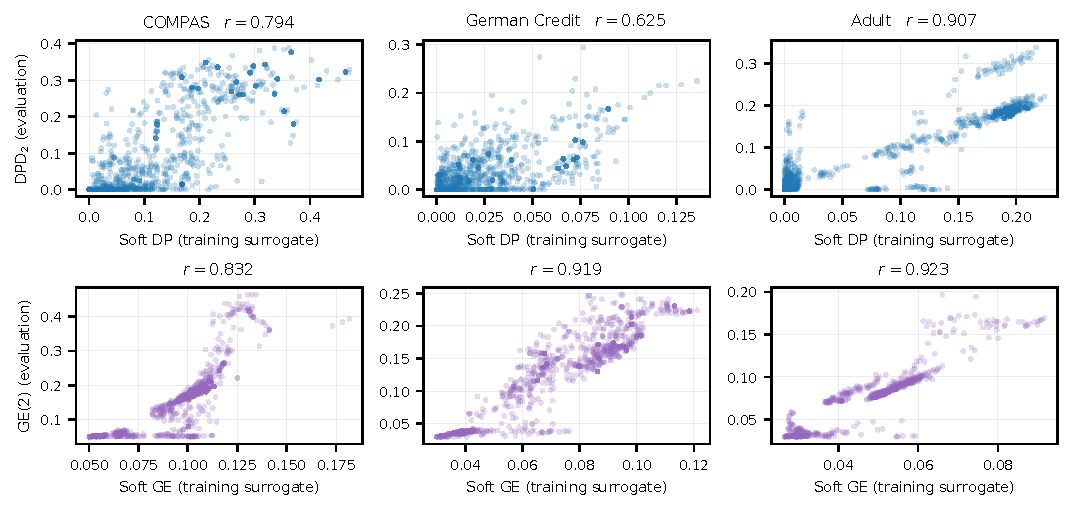
\includegraphics[width=\textwidth]{surrogate_validation.pdf}
\caption{Each training surrogate plotted against the hard evaluation metric it
stands in for, across all 2{,}940 models. Strong positive correlation is what
licenses training on the soft version and reporting the hard one.}
\label{fig:guide-surrogate}
\end{figure}

\subsection{The baseline methods}

Fairness interventions are conventionally sorted into three families. This
project covers all three.

\begin{center}
\small
\begin{tabular}{@{}llp{0.47\textwidth}@{}}
\toprule
\textbf{Family} & \textbf{Method} & \textbf{What it does} \\
\midrule
Pre-processing & Reweighing &
Give each training sample weight $w(s,y)=P(s)P(y)/P(s,y)$, making label and
sensitive attribute independent in the \emph{weighted} training distribution. \\
\addlinespace
In-processing & ExponentiatedGradient &
Reformulates constrained fair classification as a two-player game; returns a
randomised classifier. Run with Demographic Parity and with Equalized Odds. \\
\addlinespace
Post-processing & ThresholdOptimizer &
Keeps the trained model, picks a \emph{different decision threshold per group}
to satisfy the constraint. \\
\addlinespace
(none) & Random Forest, XGBoost &
No fairness intervention. These show the accuracy ceiling. \\
\bottomrule
\end{tabular}
\end{center}

\subsection{Experimental-protocol terms}

\begin{description}[leftmargin=0em,style=nextline,itemsep=5pt]

\item[Seed]
A random number controlling the train/val/test split \emph{and} weight
initialisation \emph{and} stochastic baselines. Ten seeds (0--9) means ten
independent repeats; we report mean $\pm$ std over them. This is what turns
single numbers into results with error bars.

\item[Train / validation / test split]
$60/20/20$, re-drawn per seed. Train fits the model; validation selects
hyperparameters and triggers early stopping; test is touched \textbf{only} for
final reporting.

\item[StandardScaler]
Rescale numeric features to mean $0$, std $1$. Necessary because gradient
descent behaves badly when features have wildly different scales
(\code{age} $\approx 40$, \code{capital-gain} $\approx 100{,}000$).

\item[OneHotEncoder(drop='first')]
Turn a categorical column into binary indicator columns, dropping one to avoid
perfect collinearity.

\item[Utopia-point model selection]
Among all $\alpha<1$ sweep points, pick the one minimising distance to the ideal
corner:
\[ d = \sqrt{(1-\text{val\_acc})^2 + \text{val\_DPD}_2^2} \]
Computed on \textbf{validation only}. This is a project-specific choice, not a
field standard.

\item[Degenerate-predictor guard]
A model predicting ``no'' for everyone has $\mathrm{DPD}=0$, is perfectly
``fair,'' and is useless. Any model whose validation positive rate is $<5\%$ or
$>95\%$ is excluded from selection.

\item[Wilcoxon signed-rank test]
A paired, non-parametric significance test. \emph{Paired} because seed $k$ for
the fair model and seed $k$ for the baseline share the same data split.
\emph{Non-parametric} because with ten samples you cannot credibly assume
normality.

\item[Holm correction]
Testing four metrics at once gives four chances to find a fluke. Holm's
step-down procedure adjusts the $p$-values to control the family-wise error
rate.

\item[Pareto frontier]
The set of configurations where you cannot improve accuracy without worsening
DPD, or vice versa. The ``efficient'' trade-offs.

\end{description}

\begin{example}[Why the degeneracy guard is not cosmetic]
On COMPAS, seed 0, at $\alpha = 0$ (no accuracy term at all), the trained model
records:
\begin{center}
accuracy $= 0.4526$ \qquad validation positive rate $= 0.9951$
\end{center}
The model predicts ``will re-offend'' for $99.5\%$ of people. Its demographic
parity difference is near zero, because it treats everyone identically ---
identically badly. Without the $5\%$/$95\%$ guard, model selection would rank
this as an excellent fair model.
\end{example}

\subsection{Abbreviations you will use constantly}

\begin{center}
\small
\begin{tabular}{@{}ll@{\hspace{2.5em}}ll@{}}
\toprule
\textbf{Abbr.} & \textbf{Meaning} & \textbf{Abbr.} & \textbf{Meaning} \\
\midrule
LR   & Logistic Regression        & DPD  & Demographic Parity Difference \\
MLP  & Multi-Layer Perceptron     & EOD  & Equalized Odds Difference \\
BCE  & Binary Cross-Entropy       & GE   & Generalized Entropy (index) \\
DP   & Demographic Parity         & RF   & Random Forest \\
EO   & Equalized Odds             & XGB  & XGBoost \\
ExpGrad & ExponentiatedGradient   & TPR/FPR & True/False Positive Rate \\
\bottomrule
\end{tabular}
\end{center}

\clearpage
%%%%%%%%%%%%%%%%%%%%%%%%%%%%%%%%%%%%%%%%%%%%%%%%%%%%%%%%%%%%%%%%% 3. METRICS
\section{Evaluation Metrics and Their Interpretation}

Six metrics are computed on every model. This section explains each one, how to
read its value, and --- critically --- whether any standard threshold actually
exists.

\begin{warnbox}[Read this before quoting any threshold]
There is \textbf{no universally accepted ``good'' value} for DPD, EOD, or GE.
This guide distinguishes three levels of authority:
\begin{itemize}
\item \textbf{Established standard} --- a formal, citable rule. Almost nothing
in fairness metrics qualifies.
\item \textbf{Common rule of thumb} --- widely used in practice but with no
formal backing. Label it as such in the paper.
\item \textbf{Project-specific interpretation} --- our own reading of our own
numbers.
\end{itemize}
\end{warnbox}

\subsection{Accuracy}

\textbf{What:} fraction of correct predictions.
\textbf{Direction:} higher is better.
\textbf{Range:} $0$ to $1$.

\textbf{Reference point:} the majority-class rate. Base rates in this project
are COMPAS $0.455$ (majority-class $\approx 0.545$), German $0.300$
($\approx 0.70$), Adult $0.248$ ($\approx 0.752$). A model must beat that to be
doing anything at all.

\textbf{Standard?} Accuracy itself is universal; there is \textbf{no universal
``good'' accuracy}. What exists is \emph{literature-typical} performance per
dataset --- COMPAS models land at $\approx 0.66$--$0.70$, Adult
$\approx 0.84$--$0.87$, German $\approx 0.72$--$0.77$.

\subsection{DPD --- Demographic Parity Difference}

\textbf{Stands for:} Demographic Parity Difference (also: statistical parity
difference).

\textbf{Measures:} the largest gap in \textbf{selection rate} (fraction
predicted positive) between sensitive groups:
\begin{equation}
\mathrm{DPD} = \max_g P(\hat y = 1 \mid S = g) - \min_g P(\hat y = 1 \mid S = g)
\end{equation}
It \textbf{ignores the true labels entirely} --- it only asks who gets flagged,
not who deserved it.

\textbf{Direction:} lower is better. \textbf{Range:} $0$ to $1$. Zero means
every group is flagged at an identical rate.

\begin{warnbox}[Is there a standard threshold? No.]
What people \emph{do} cite:
\begin{itemize}
\item \textbf{The four-fifths rule / 80\% rule} (US EEOC, \emph{Uniform
Guidelines on Employee Selection Procedures}, 1978) --- a legal rule of thumb
for adverse impact. But it is a \textbf{ratio} test
($\min\text{ rate}/\max\text{ rate} \ge 0.8$), \textbf{not a difference test}.
It does not translate to a DPD threshold without knowing the base selection
rate. Cite it for context; do \emph{not} claim ``DPD $<0.2$ passes the 80\%
rule'' --- that is only true if the maximum selection rate happens to be $1.0$.
\item \textbf{Common informal practice:} DPD $<0.05$ is treated as ``close to
parity,'' $0.05$--$0.10$ as modest disparity, $>0.10$ as substantial. This is a
\emph{convention}, not a standard.
\end{itemize}
\end{warnbox}

\subsubsection{The two variants in this project}
\begin{itemize}
\item \code{Demographic Parity Difference} --- computed over \textbf{all} groups.
\item \code{DPD (Largest 2 Groups)}, written \dpdtwo{} --- restricted to the two
largest groups. On COMPAS that is African-American ($n=3175$) vs Caucasian
($n=2103$), ProPublica's focal comparison. On German and Adult (two groups
each) the two variants are \textbf{identical by construction}.
\end{itemize}

\begin{example}[Why the largest-2 variant exists]
COMPAS has six race groups and the small ones are tiny: Asian $n=31$, Native
American $n=11$ across the \emph{whole} dataset --- roughly $6$ and $2$ people
in a 1{,}235-row test split. A $\max-\min$ over all groups is then pinned by a
handful of individuals and swings wildly. The evidence is in our own results:
\begin{center}
\begin{tabular}{@{}lcc@{}}
\toprule
COMPAS, LR baseline & mean & std \\
\midrule
DPD (all six groups)  & $0.608$ & $\pm 0.211$ \\
\dpdtwo{} (two largest) & $0.304$ & $\pm 0.049$ \\
\bottomrule
\end{tabular}
\end{center}
The standard deviation is over four times larger for the all-groups version.
That is why \dpdtwo{} is the primary metric --- and this table \emph{is} the
justification to put in the paper.
\end{example}

\subsection{EOD --- Equalized Odds Difference}

\textbf{Measures:} whether the model's \emph{error rates} are equal across
groups. Computed as the larger of \{max$-$min true-positive-rate gap,
max$-$min false-positive-rate gap\}. Unlike DPD it \emph{does} use the true
labels --- it asks whether the model is equally accurate for each group, not
whether it selects them equally often.

\textbf{Direction:} lower is better. \textbf{Range:} $0$ to $1$.
\textbf{Standard threshold?} \textbf{No} --- same situation as DPD.

\begin{keybox}[The relationship that drives our biggest result]
DPD and EOD are \textbf{mathematically incompatible} whenever base rates differ
across groups. Our data has exactly that: Adult female base rate $0.114$ vs
male $0.312$; COMPAS African-American $0.523$ vs Caucasian $0.391$. So
\textbf{driving DPD to zero must push EOD up.} Our Adult results show this
precisely.
\end{keybox}

\begin{warnbox}[COMPAS EOD is unreliable in the current code]
EOD is computed over \textbf{all} groups, without the largest-2 restriction
that was applied to DPD. So COMPAS EOD inherits exactly the tiny-group noise
problem --- which is why every COMPAS EOD is $\approx 0.64$--$0.83$ with std
$\approx 0.15$--$0.22$, and why \emph{no} COMPAS EOD comparison reaches
significance. Either add a largest-2 EOD, or explicitly caveat the column. Do
not report it as a clean finding.
\end{warnbox}

\subsection{GE(2) --- Generalized Entropy Index (labelled ``Theil'' in the code)}

\textbf{What it is:} inequality of the benefit vector $b = 1 + \hat y - y$,
measured with the generalized entropy index of order $2$:
\begin{equation}
\getwo = \frac{1}{2n}\sum_i\left[\left(\frac{b_i}{\bar b}\right)^{2} - 1\right]
       = \frac{\mathrm{Var}(b)}{2\,\bar b^{\,2}}
\end{equation}

\textbf{Direction:} lower is better. \textbf{Range:} $0$ to $\infty$ in
principle; $0$ means perfectly equal benefit (a perfect classifier, since every
$b=1$).

\begin{warnbox}[Naming error to fix before submitting]
\file{IndividualFairness.py} defines \code{theil\_index} as AIF360's
\code{generalized\_entropy\_error(..., alpha=2)}. That is \textbf{backwards
relative to the standard definition}. AIF360's own docstring states: a value of
$0$ is the mean log deviation, \textbf{$1$ is the Theil index}, and $2$ is half
the squared coefficient of variation.

So everything the project calls ``Theil Index'' is really \textbf{GE($\alpha=2$)}.
\textbf{No number is wrong} --- GE(2) is a perfectly standard inequality index,
and crucially it is the \emph{same} index the SoftGE surrogate optimises (also
$\alpha=2$), so training and evaluation are consistent. But the \textbf{label}
must change, or a reviewer familiar with Speicher et al.\ will flag it
immediately. The paper produced alongside this guide already uses
\textbf{GE(2)} throughout.
\end{warnbox}

\textbf{What it actually captures on hard predictions:} with binary
predictions, $b \in \{0,1,2\}$ only. So GE(2) here is a \textbf{function of the
false-positive and false-negative counts alone}. It measures how much error
there is and how it splits between the two error types --- not, strictly, whether
\emph{similar individuals} got similar treatment. This is the standard Speicher
et al.\ operationalisation, so it is defensible, but be precise: it is an
\emph{inequality-of-outcomes} measure, not a Lipschitz-style ``similar
individuals treated similarly'' measure.

\textbf{Standard threshold?} \textbf{None whatsoever.} GE has no absolute
interpretation. It is meaningful \textbf{only comparatively} --- model A versus
model B on the same dataset. Say this plainly in the paper rather than implying
a range.

\subsection{Gini Coefficient}

\textbf{What it is supposed to be:} the classic economics inequality measure,
from the Lorenz curve. $0 =$ perfect equality, $1 =$ maximum inequality.

\begin{warnbox}[This metric carries no fairness information]
\file{IndividualFairness.py} applies the Lorenz/Gini construction to
\code{y\_pred} directly. Since \code{y\_pred} is a vector of 0s and 1s, this
reduces \textbf{exactly} to
\[ \mathrm{Gini} = 1 - \text{positive prediction rate} \]
Verified numerically to four decimal places on three random vectors (positive
rate $0.3270 \to$ Gini $0.6730$; $0.2045 \to 0.7955$; $0.4700 \to 0.5300$), and
consistent with the result tables (German LR baseline Gini $0.869$ implies a
positive rate of $0.131$ against a base rate of $0.30$ --- plausible
under-prediction on an imbalanced dataset).

\textbf{Recommendation:} either \textbf{drop it} from the paper, or
\textbf{relabel it} as ``selection rate (reported as $1-$Gini)'' --- which is
genuinely useful, since it is exactly the quantity the degeneracy guard
watches. What you must not do is present it as an independent
individual-fairness metric.
\end{warnbox}

\subsection{Soft DP / Soft GE}

Logged per sweep point, computed on \emph{test probabilities}. These are not
evaluation metrics --- they exist solely for the surrogate-validation scatter
(Figure~\ref{fig:guide-surrogate}). Keep them in supplementary material.

\subsection{Summary table}

\begin{center}
\scriptsize
\renewcommand{\arraystretch}{1.3}
\setlength{\tabcolsep}{3.5pt}
\begin{tabular}{@{}L{0.098\textwidth} L{0.205\textwidth} c L{0.055\textwidth} L{0.195\textwidth} L{0.245\textwidth}@{}}
\toprule
\textbf{Metric} & \textbf{Meaning (plain)} & \textbf{Dir.} & \textbf{Range}
& \textbf{Standard?} & \textbf{How we interpret our result} \\
\midrule

\textbf{Accuracy} & \% correct & $\uparrow$ & $0$--$1$ &
No. Compare to majority-class rate and dataset literature &
COMPAS ${\approx}0.68$, Adult ${\approx}0.85$, German ${\approx}0.73$ --- all
literature-typical \\

\textbf{DPD} (all groups) & Max$-$min selection rate over all groups &
$\downarrow$ & $0$--$1$ &
\textbf{No.} 80\% rule is a \emph{ratio} test, not a difference test &
On COMPAS dominated by tiny-group noise --- report as secondary only \\

\textbf{\dpdtwo{}} & Same, restricted to the two biggest groups &
$\downarrow$ & $0$--$1$ &
\textbf{No.} ``${<}0.05$ = near parity'' is convention, not standard &
\textbf{Primary group-fairness metric.} Stable across seeds \\

\textbf{EOD} & Max gap in TPR \emph{or} FPR across groups &
$\downarrow$ & $0$--$1$ &
\textbf{No.} ``${<}0.1$'' is convention only &
Mathematically opposed to DPD when base rates differ.
\textbf{COMPAS values unreliable} \\

\textbf{\getwo{}} & Inequality of benefit $b = 1{+}\hat y{-}y$ &
$\downarrow$ & $0$--$\infty$ &
\textbf{None. Comparative only} &
\textbf{Primary individual-fairness metric.} Only meaningful vs another model
on the same data \\

\textbf{Gini} & \emph{As implemented:} exactly $1-$selection rate &
--- & $0$--$1$ & n/a &
\textbf{Not an independent fairness metric.} Drop or relabel \\

\textbf{Soft DP / Soft GE} & Differentiable training surrogates &
$\downarrow$ & --- & n/a &
Supplementary: validates soft ${\approx}$ hard ($r = 0.63$--$0.92$) \\

\bottomrule
\end{tabular}
\\[4pt]
\footnotesize $\uparrow$ = higher is better, $\downarrow$ = lower is better.
\end{center}

%%%%%%%%%%%%%%%%%%%%%%%%%%%%%%%%%%%%%%%%%%%%%%%%%%%%%%%%%%%%% 4. METHODOLOGY
\section{Methodology, Step by Step}

\subsection{Step 1 --- Dataset selection and loading}

Three datasets, chosen because together they are the field-standard trio for
tabular fairness work. Actual figures, read from the loaders:

\begin{center}
\small
\begin{tabular}{@{}lccc@{}}
\toprule
 & \textbf{COMPAS} & \textbf{German Credit} & \textbf{Adult} \\
\midrule
Samples $n$            & $6{,}172$ & $1{,}000$ & $45{,}222$ \\
Target ($y=1$)         & re-offended & \textbf{bad} credit & income $>$\$50K \\
Sensitive attribute    & race & Sex & sex \\
Number of groups       & $6$ & $2$ & $2$ \\
Overall base rate      & $0.455$ & $0.300$ & $0.248$ \\
Encoded features       & $12$ & $21$ & $\approx 79$ \\
\midrule
\multicolumn{4}{@{}l}{\textit{Group sizes and per-group base rates}} \\
Largest group  & Afr.-Am.\ $3{,}175$ ($0.523$) & male $690$ ($0.277$) & Male $30{,}527$ ($0.312$) \\
2nd largest    & Caucasian $2{,}103$ ($0.391$) & female $310$ ($0.352$) & Female $14{,}695$ ($0.114$) \\
Others         & Hisp.\ $509$, Other $343$, & --- & --- \\
               & \textbf{Asian 31, Nat.Am.\ 11} & & \\
\bottomrule
\end{tabular}
\end{center}

\textbf{Why these three:} they span three domains (criminal justice, credit,
income), two sensitive attributes (race, sex), and three orders of magnitude of
sample size --- exactly what RQ2 needs to test consistency.

\textbf{Why the differing base rates matter:} they are the \emph{reason} DPD and
EOD conflict. Adult's female-vs-male base rate gap ($0.114$ vs $0.312$, a factor
of $2.7$) is the mechanical driver of our most striking result.

\subsection{Step 2 --- The COMPAS leakage fix}

We apply ProPublica's standard row filters:
\begin{itemize}
\item \code{days\_b\_screening\_arrest} within $\pm30$ days
\item \code{is\_recid} $\ne -1$
\item \code{c\_charge\_degree} $\ne$ \code{O}
\item \code{score\_text} $\ne$ \code{N/A}
\end{itemize}
Features used:
\code{age}, \code{sex}, \code{juv\_fel\_count}, \code{juv\_misd\_count},
\code{juv\_other\_count}, \code{priors\_count}, \code{c\_charge\_degree},
\code{race}.

\begin{keybox}[This is a genuine methodological contribution]
An earlier version of this project included a feature
$\code{duration} = \code{end} - \code{start}$ that correlated $\boldsymbol{-0.78}$
with the target. That correlation is \textbf{mechanical, not predictive}:
re-offending truncates the observation window, so short duration $\Rightarrow$
re-offended, almost by definition. That is \textbf{label leakage} --- the model
was reading the answer off the feature.

Removing it drops COMPAS accuracy to the literature-typical
$\approx 0.67$--$0.68$. \textbf{This is a correction, not a regression.} Frame it
as a soundness contribution in the paper.
\end{keybox}

\subsection{Step 3 --- Preprocessing}

Per seed:
\begin{enumerate}
\item Split $60/20/20$ into train/validation/test. (Note: splits are
\emph{not} stratified --- worth a sentence in the paper.)
\item Extract the sensitive column per split; build integer group codes with
\textbf{one shared category mapping across all splits} so group IDs mean the
same thing everywhere. This matters --- the torch loss indexes by these codes.
\item Fit the \code{ColumnTransformer} \textbf{on train only}, apply to
val/test --- correct, no leakage:
  \begin{itemize}
  \item numeric $\to$ \code{StandardScaler}
  \item categorical $\to$ \code{OneHotEncoder(drop='first', handle\_unknown='ignore')}
  \end{itemize}
\item Convert to torch tensors.
\end{enumerate}

\begin{warnbox}[There is no feature-engineering step --- say so]
No interaction terms, no binning, no feature selection. Features are used as
published. This is \emph{appropriate} --- the paper is about the loss function,
and inventing features would confound the comparison. But state it explicitly
rather than leaving a gap where a ``feature engineering'' section would be.
\end{warnbox}

\subsection{Step 4 --- The composite loss}

Equation~\eqref{eq:composite}, with SoftDP and SoftGE as defined earlier. Two
bugs from the legacy code are fixed here, and both belong in the paper's
reproducibility discussion:

\begin{enumerate}
\item \textbf{Gradient flow.} The original computed fairness terms via
fairlearn/aif360 on the detached array
\begin{center}\code{y\_pred.round().detach().numpy()}\end{center}
The \code{.detach()} severs the autograd graph --- \textbf{only BCE ever
produced gradients}, so $\alpha$ and $\beta$ had almost no effect on the learned model.
That is why the legacy heatmaps were flat in $\beta$. Every term is now computed
in torch on raw probabilities.
\item \textbf{Double sigmoid.} The old model applied sigmoid in \code{forward}
and the loss applied it again. Now models return logits and the loss uses
\code{binary\_cross\_entropy\_with\_logits}.
\end{enumerate}

\begin{example}[Putting a number through the composite loss]
Suppose at some point in training, on the training batch:
\[
\mathrm{BCE} = 0.62, \qquad \mathrm{SoftDP} = 0.18, \qquad \mathrm{SoftGE} = 0.09
\]
Compare two settings of the dial at the same fairness pressure
$\alpha = 0.75$ (so $1-\alpha = 0.25$):

\medskip
\textbf{$\beta = 1$ (group-only):}
\[
\mathcal{L} = 0.75(0.62) + 0.25\big[1(0.18) + 0(0.09)\big]
            = 0.465 + 0.045 = \mathbf{0.510}
\]

\textbf{$\beta = 0$ (individual-only):}
\[
\mathcal{L} = 0.75(0.62) + 0.25\big[0(0.18) + 1(0.09)\big]
            = 0.465 + 0.0225 = \mathbf{0.4875}
\]

\textbf{$\beta = 0.5$ (blend):}
\[
\mathcal{L} = 0.465 + 0.25\big[0.5(0.18) + 0.5(0.09)\big]
            = 0.465 + 0.03375 = \mathbf{0.4988}
\]

Same accuracy term in all three; only the \emph{composition} of the fairness
penalty changes. Gradient descent therefore pushes the model in a different
direction for each $\beta$ --- which is the entire mechanism the study
exploits.
\end{example}

\subsection{Step 5 --- Training}

Adam (lr $0.01$, weight decay $10^{-4}$), full-batch, up to 300 epochs, early
stopping on \textbf{validation composite loss} with patience 20, best weights
restored from a deep copy.

Note that early stopping monitors the \emph{composite} loss at that
$(\alpha,\beta)$ --- not plain BCE. This is the right choice (you select the best
model for the objective you are actually optimising), but it means the stopping
criterion shifts as you move across the grid. Mention it.

\subsection{Step 6 --- The sweep}

For each of $7\alpha \times 7\beta = 49$ combinations, per architecture (2), per
dataset (3), per seed (10):

\begin{itemize}
\item Set \code{torch.manual\_seed(seed)} and \code{np.random.seed(seed)}
before instantiating the model $\Rightarrow$ identical initialisation across
grid points within a seed, so differences are attributable to $(\alpha,\beta)$,
not initialisation luck.
\item Train (or load a cached checkpoint).
\item Predict on test, threshold at $0.5$, compute all six metrics.
\item Also record validation accuracy, validation \dpdtwo{}, validation positive
rate (for selection and the degeneracy guard), soft metrics, and training time.
\end{itemize}

\begin{center}
\textbf{Total: $49 \times 2 \times 3 \times 10 = 2{,}940$ trained models.}
\end{center}

\subsection{Step 7 --- Model selection}

Validation-only, in three steps:
\begin{enumerate}
\item Keep $\alpha < 1$ (must have \emph{some} fairness weight).
\item Keep validation positive rate $\in [0.05, 0.95]$ (degeneracy guard).
\item Minimise $\sqrt{(1-\text{val\_acc})^2 + \text{val\_DPD}_2^2}$.
\item Test metrics reported only, \textbf{never used for selection}.
\end{enumerate}

Which $(\alpha, \beta)$ actually got picked, across ten seeds --- this is itself
a result:

\begin{center}
\small
\begin{tabular}{@{}llcc@{}}
\toprule
\textbf{Dataset} & \textbf{Model} & \textbf{Distinct configs / 10 seeds} & \textbf{Mean $\beta$} \\
\midrule
COMPAS & Fair LR  & $5$  & $0.63$ \\
COMPAS & Fair MLP & $5$  & $0.60$ \\
German & Fair LR  & $8$  & $0.19$ \\
German & Fair MLP & $\mathbf{10}$ & $0.41$ \\
Adult  & Fair LR  & $4$  & $0.58$ \\
Adult  & Fair MLP & $3$  & $0.65$ \\
\bottomrule
\end{tabular}
\end{center}

German is unstable: the MLP picks a \emph{different} configuration in every
single seed. That instability is a finding, analysed in
Section~\ref{sec:guide-german}.

\subsection{Step 8 --- Baselines and Step 9 --- Aggregation}

All baselines are fit on the same seed's training split and evaluated on the
same test split. Then the ten per-seed CSVs are concatenated, and for each
(fair model, baseline) pair we run a \textbf{paired Wilcoxon signed-rank test}
across seeds per metric, \textbf{Holm-corrected} across the metric family
\{Accuracy, \dpdtwo{}, EOD, \getwo{}\}.

\begin{warnbox}[A statistical detail to get right]
With $n=10$ seeds, the smallest two-sided $p$-value a Wilcoxon test can produce
is $2^{-9} \approx 0.00195$. Report it as $p = 0.002$. Do \textbf{not} write
``$p < 0.001$'' --- that is not attainable at this sample size, and it means
every single seed moved in the same direction.
\end{warnbox}

\subsection{Libraries used}

\begin{center}
\small
\begin{tabular}{@{}ll@{}}
\toprule
\textbf{Library} & \textbf{Used for} \\
\midrule
PyTorch & models + the differentiable composite loss \\
scikit-learn & preprocessing, splits, LR/RF, accuracy \\
fairlearn & DPD, EOD, ExponentiatedGradient, ThresholdOptimizer \\
AIF360 & generalized entropy index \\
xgboost & XGBoost accuracy reference \\
scipy & Wilcoxon signed-rank test \\
pandas / numpy & data handling \\
matplotlib / seaborn & figures \\
\bottomrule
\end{tabular}
\end{center}

\clearpage
%%%%%%%%%%%%%%%%%%%%%%%%%%%%%%%%%%%%%%%%%%%%%%%%%%%%%%%%%%%%%%%% 5. FLOWCHART
\section{Methodology Flowchart}

Figure~\ref{fig:guide-pipeline} shows the complete pipeline as actually
implemented. Note that the generic template
(data $\to$ preprocessing $\to$ feature engineering $\to$ model $\to$ evaluation)
is modified in two ways for this project: there is \textbf{no feature
engineering stage} (deliberate --- features are used as published), and the
model stage \textbf{branches} into the sweep and the baselines before rejoining
at evaluation.

\begin{figure}[htbp]
\centering
\begin{tikzpicture}[
  every node/.style={font=\small},
  box/.style={rectangle, rounded corners=2pt, draw=ink!70, thick,
              text width=0.72\textwidth, align=center, inner sep=5pt,
              minimum height=9mm, fill=black!3},
  hi/.style={box, fill=accentlt, draw=accent, very thick},
  sm/.style={rectangle, rounded corners=2pt, draw=ink!70, thick,
             text width=0.335\textwidth, align=center, inner sep=5pt,
             minimum height=14mm, fill=black!3},
  ar/.style={-{Latex[length=2.6mm]}, thick, draw=ink!75}
]
\node[box] (data) {\textbf{DATA SOURCES}\\[1pt]
  \footnotesize COMPAS ($n{=}6{,}172$, race) \textbullet\ German Credit
  ($n{=}1{,}000$, sex) \textbullet\ Adult ($n{=}45{,}222$, sex)};

\node[hi, below=5mm of data] (filt) {\textbf{SOUNDNESS FILTERS}\\[1pt]
  \footnotesize ProPublica row filters \textbullet\ \textbf{drop leaking
  \code{duration}} ($r={-}0.78$, mechanical)};

\node[box, below=5mm of filt] (split) {\textbf{PER-SEED SPLIT} (seeds 0--9)\\[1pt]
  \footnotesize 60\% train / 20\% validation / 20\% test};

\node[box, below=5mm of split] (prep) {\textbf{PREPROCESSING} (fit on TRAIN only)\\[1pt]
  \footnotesize numeric $\to$ StandardScaler \textbullet\ categorical $\to$
  OneHot(drop=first) \textbullet\ sensitive attr $\to$ shared integer codes};

\node[sm] (sweep) at ([xshift=-0.185\textwidth, yshift=-16mm]prep.south)
  {\textbf{$\boldsymbol{\alpha \times \beta}$ SWEEP}\\[1pt]
   \footnotesize $7\times7$ grid, 2 architectures\\
   \footnotesize Adam, full-batch, early stop\\
   \footnotesize \textbf{2{,}940 models}};

\node[sm] (base) at ([xshift=0.185\textwidth, yshift=-16mm]prep.south)
  {\textbf{BASELINES}\\[1pt]
   \footnotesize Reweighing (pre)\\
   \footnotesize ExpGrad DP/EO (in), ThreshOpt (post)\\
   \footnotesize RandomForest, XGBoost};

\node[hi] (sel) at ([yshift=-44mm]prep.south)
  {\textbf{MODEL SELECTION --- VALIDATION SET ONLY}\\[1pt]
   \footnotesize keep $\alpha<1$ \textbullet\ guard $0.05 \le$ pos.\ rate $\le 0.95$
   \textbullet\ $\arg\min \sqrt{(1-\mathrm{acc})^2 + \mathrm{DPD}_2^2}$};

\node[box, below=5mm of sel] (eval) {\textbf{EVALUATION ON TEST} (threshold $0.5$)\\[1pt]
  \footnotesize Accuracy \textbullet\ DPD (all) \textbullet\ \dpdtwo{}
  \textbullet\ EOD \textbullet\ \getwo{} \textbullet\ Gini};

\node[box, below=5mm of eval] (agg) {\textbf{AGGREGATION OVER 10 SEEDS}\\[1pt]
  \footnotesize mean $\pm$ std \textbullet\ paired Wilcoxon signed-rank
  \textbullet\ Holm correction};

\node[hi, below=5mm of agg] (res) {\textbf{RESULTS \& CONCLUSION}\\[1pt]
  \footnotesize Pareto frontiers \textbullet\ $\beta$ cross-effect curves
  \textbullet\ ablation \textbullet\ master comparison\\
  \footnotesize $\Rightarrow$ empirical map of the group $\leftrightarrow$
  individual fairness trade-off};

\draw[ar] (data) -- (filt);
\draw[ar] (filt) -- (split);
\draw[ar] (split) -- (prep);
\draw[ar] (prep.south) -- ++(0,-5mm) -| (sweep.north);
\draw[ar] (prep.south) -- ++(0,-5mm) -| (base.north);
\draw[ar] (sweep.south) |- ([yshift=-6mm]sweep.south) -| (sel.north);
\draw[ar] (base.south)  |- ([yshift=-6mm]base.south)  -| (sel.north);
\draw[ar] (sel) -- (eval);
\draw[ar] (eval) -- (agg);
\draw[ar] (agg) -- (res);
\end{tikzpicture}
\caption{The complete pipeline. Highlighted boxes are the three steps that most
affect the validity of the conclusions.}
\label{fig:guide-pipeline}
\end{figure}

\clearpage

%%%%%%%%%%%%%%%%%%%%%%%%%%%%%%%%%%%%%%%%%%%%%%%%%%%%%%%%%%%%%%%%%%%% 6. RESULTS
\section{Understanding Our Results}

\subsection{Headline: the \texorpdfstring{$\beta$}{beta} ablation --- this is the paper}

This is the cleanest evidence for RQ1. It holds $\alpha$ fixed and moves $\beta$
between the extremes, so the \emph{amount} of fairness pressure is constant and
only its \emph{composition} changes.

\begin{center}
\small
\textbf{COMPAS, Logistic Regression ($\alpha = 0.75$)}\\[3pt]
\begin{tabular}{@{}lccc@{}}
\toprule
\textbf{Variant} & \textbf{Accuracy} & \textbf{\dpdtwo{}} $\downarrow$ & \textbf{\getwo{}} $\downarrow$ \\
\midrule
No fairness ($\alpha{=}1$) & $0.676 \pm 0.012$ & $0.304 \pm 0.049$ & $0.191 \pm 0.012$ \\
\rowcolor{goodlt} SoftGE only ($\beta{=}0$) & $0.674 \pm 0.012$ & $\mathbf{0.305} \pm 0.049$ & $\mathbf{0.181} \pm 0.010$ \\
\rowcolor{warnlt} SoftDP only ($\beta{=}1$) & $0.650 \pm 0.014$ & $\mathbf{0.067} \pm 0.053$ & $\mathbf{0.217} \pm 0.021$ \\
Blend ($\beta{=}0.5$) & $0.660 \pm 0.021$ & $0.092 \pm 0.065$ & $0.204 \pm 0.026$ \\
\bottomrule
\end{tabular}
\end{center}

\textbf{Read it row by row --- this is the whole story:}
\begin{itemize}
\item Optimising \textbf{individual fairness alone} ($\beta=0$): \getwo{}
improves $0.191 \to 0.181$ ($-5\%$). \dpdtwo{} is \textbf{completely unmoved}:
$0.304 \to 0.305$. It does nothing for group fairness.
\item Optimising \textbf{group fairness alone} ($\beta=1$): \dpdtwo{} collapses
$0.304 \to 0.067$ ($\mathbf{-78\%}$). But \getwo{} gets \textbf{worse}:
$0.191 \to 0.217$ ($+14\%$) --- \emph{worse than doing nothing at all}.
\item The blend sits in between on both.
\end{itemize}

The same pattern appears on Adult, and it is statistically significant. Full
ablation with Holm-corrected significance:

\begin{center}
\scriptsize
\renewcommand{\arraystretch}{1.15}
\begin{tabular}{@{}llcccc@{}}
\toprule
\textbf{Dataset} & \textbf{Variant} & \textbf{Accuracy} & \textbf{\dpdtwo{}} & \textbf{EOD} & \textbf{\getwo{}} \\
\midrule
\multirow{3}{*}{COMPAS}
 & No fairness            & $0.676$ & $0.304$ & $0.789$ & $0.191$ \\
 & SoftGE only ($\beta{=}0$) & $0.674$ & $0.305$\ \textsc{ns} & $0.811^{*}$ & $\mathbf{0.181^{**}}$ \\
 & SoftDP only ($\beta{=}1$) & $0.650^{**}$ & $\mathbf{0.067^{**}}$ & $0.681$\ \textsc{ns} & $\mathbf{0.217^{**}}$ \\
\midrule
\multirow{3}{*}{German}
 & No fairness            & $0.730$ & $0.046$ & $0.090$ & $0.175$ \\
 & SoftGE only ($\beta{=}0$) & $0.730$\ \textsc{ns} & $0.050$\ \textsc{ns} & $0.106$\ \textsc{ns} & $0.170$\ \textsc{ns} \\
 & SoftDP only ($\beta{=}1$) & $0.731$\ \textsc{ns} & $0.029$\ \textsc{ns} & $0.103$\ \textsc{ns} & $0.173$\ \textsc{ns} \\
\midrule
\multirow{3}{*}{Adult}
 & No fairness            & $0.845$ & $0.184$ & $0.107$ & $0.084$ \\
 & SoftGE only ($\beta{=}0$) & $0.845$\ \textsc{ns} & $\mathbf{0.189^{**}}$ & $0.113^{*}$ & $\mathbf{0.083^{*}}$ \\
 & SoftDP only ($\beta{=}1$) & $0.833^{**}$ & $\mathbf{0.040^{**}}$ & $\mathbf{0.246^{**}}$ & $\mathbf{0.094^{**}}$ \\
\bottomrule
\end{tabular}
\\[3pt]
\footnotesize Logistic regression. $^{**}p_{\mathrm{Holm}}<0.01$,
$^{*}p_{\mathrm{Holm}}<0.05$, \textsc{ns} $=$ not significant.
\end{center}

\begin{keybox}[The result, stated precisely: a double dissociation]
\begin{enumerate}
\item Group fairness $\leftarrow$ group objective: \textbf{strong} effect
($-78\%$ DPD, $p_{\mathrm{Holm}} = 0.008$, consistent across datasets and
architectures).
\item Individual fairness $\leftarrow$ individual objective: \textbf{weak but
real and significant} effect ($-5\%$ GE, $p_{\mathrm{Holm}} \le 0.012$).
\item \textbf{The cross-effects are negative in both directions.} Optimising
group fairness significantly \emph{harms} individual fairness. Optimising
individual fairness leaves group fairness unchanged (COMPAS) or significantly
\emph{worse} (Adult).
\end{enumerate}
\textbf{Is this good? Yes --- it is an excellent result}, because it is clean,
replicated, and significant in both directions.
\end{keybox}

\begin{figure}[htbp]
\centering
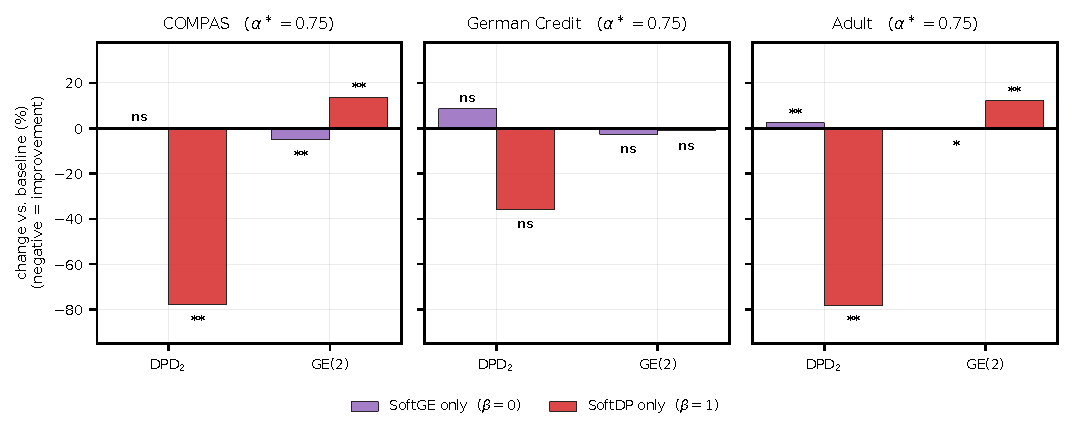
\includegraphics[width=\textwidth]{double_dissociation.pdf}
\caption{The double dissociation as percentage change from baseline. Purple
($\beta=0$, individual-only) lowers GE(2) but not DPD. Red ($\beta=1$,
group-only) crushes DPD but raises GE(2). German shows no significant movement
in either direction.}
\end{figure}

\textbf{Why the asymmetry (effect 1 strong, effect 2 weak)?} This is itself a
finding, not a flaw. SoftDP directly manipulates a quantity the model controls
freely --- the group-wise mean of predicted probabilities --- and can shift it
by moving the decision surface, which costs little accuracy. SoftGE is bounded
by irreducible prediction error: benefit is equal only when everyone is
predicted equally correctly, so you \emph{cannot} equalise benefit without
actually being more accurate. On COMPAS, where the accuracy ceiling is about
$0.68$, there is very little room.

\subsection{The \texorpdfstring{$\beta$}{beta} cross-effect curves}

\begin{figure}[htbp]
\centering
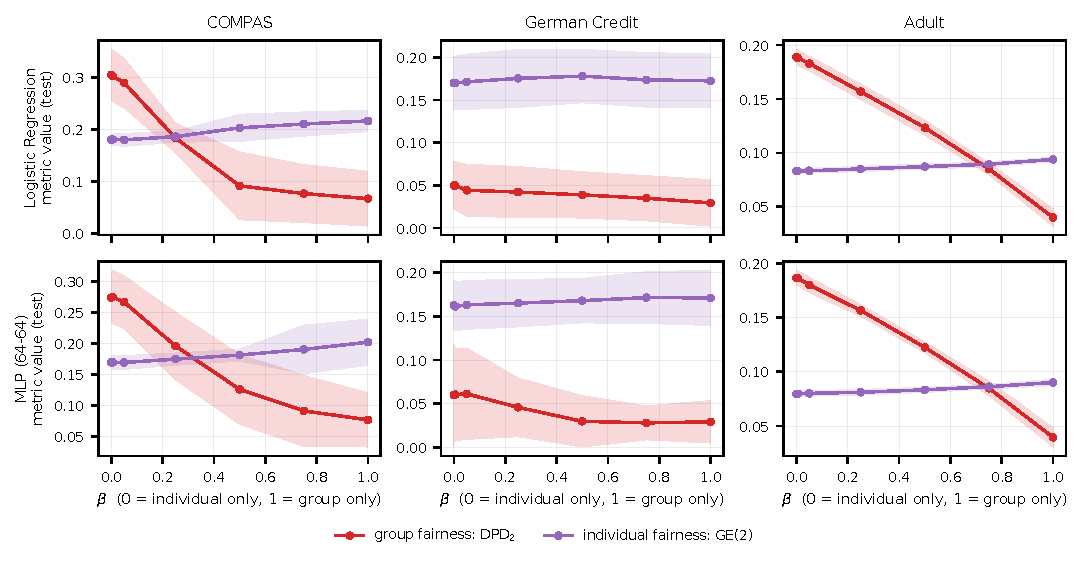
\includegraphics[width=\textwidth]{beta_cross_effect.pdf}
\caption{The trade-off seen continuously. As $\beta$ moves from individual-only
(0) to group-only (1), the group metric (red) falls and the individual metric
(purple) rises. The \textbf{crossing curves} on COMPAS and Adult are the
result; German is flat because there is almost no disparity to remove.}
\end{figure}

\subsection{Fair model versus baseline (the selected models)}

Holm-corrected $p$-values for the selected fair model against its matched
baseline:

\begin{center}
\small
\begin{tabular}{@{}llcccc@{}}
\toprule
\textbf{Dataset} & \textbf{Arch} & \textbf{Accuracy} & \textbf{\dpdtwo{}} & \textbf{EOD} & \textbf{\getwo{}} \\
\midrule
COMPAS & LR  & $\mathbf{0.008}$ & $\mathbf{0.008}$ & $0.232$ & $\mathbf{0.027}$ \\
COMPAS & MLP & $\mathbf{0.018}$ & $\mathbf{0.008}$ & $0.863$ & $0.863$ \\
German & LR  & $1.000$ & $1.000$ & $1.000$ & $0.422$ \\
German & MLP & $1.000$ & $1.000$ & $1.000$ & $1.000$ \\
Adult  & LR  & $\mathbf{0.008}$ & $\mathbf{0.008}$ & $\mathbf{0.008}$ & $\mathbf{0.008}$ \\
Adult  & MLP & $\mathbf{0.008}$ & $\mathbf{0.008}$ & $\mathbf{0.008}$ & $\mathbf{0.008}$ \\
\bottomrule
\end{tabular}
\end{center}

\subsubsection{COMPAS --- good result}
\dpdtwo{} drops $0.304 \to 0.061$ (LR), an \textbf{80\% reduction}, at a cost of
$1.5$ accuracy points ($0.676 \to 0.661$). Both significant. \getwo{} worsens
$0.191 \to 0.200$, also significant. \textbf{Verdict: good.} A five-fold
fairness improvement for $1.5$ points of accuracy is a favourable exchange rate
by the standards of this literature, and the individual-fairness cost is
measured rather than hidden.

\subsubsection{Adult --- the strongest and most interpretable result}
\dpdtwo{} $0.184 \to 0.021$ ($\mathbf{-89\%}$), accuracy $0.845 \to 0.830$
($-1.5$ points), EOD $0.107 \to \mathbf{0.279}$ ($2.6\times$ \emph{worse}),
\getwo{} $0.084 \to 0.095$. All four significant, all four moving in the same
direction across all ten seeds.

\begin{keybox}[Why Adult's ``bad'' EOD number is the best result in the paper]
Adult's base rates are $0.114$ (female) vs $0.312$ (male) --- a $2.7\times$ gap.
Theory says you cannot have demographic parity and equalized odds
simultaneously under unequal base rates. Your experiment shows exactly that, at
the predicted magnitude. This is a \textbf{textbook confirmation}, and you
should present it as one. The exchange rate is roughly one point of DPD for
$1.1$ points of EOD.
\end{keybox}

\subsection{The German Credit null result --- and its real cause}
\label{sec:guide-german}

On German, \textbf{nothing is significant} --- not one metric, not one
architecture. This must be reported as a null result, not buried. But the
common-sense explanation (``the dataset is small'') is only half right, and the
naive explanation (``the method doesn't work here'') is \textbf{wrong}.

\subsubsection{The decisive diagnostic}
Model selection ranks configurations by \emph{validation} DPD. So: does
validation DPD predict test DPD?

\begin{center}
\small
\begin{tabular}{@{}lccc@{}}
\toprule
\textbf{Dataset} & $r$(val DPD, test DPD) & \textbf{SNR} & \textbf{acc:DPD term ratio} \\
\midrule
COMPAS & $0.94$ & $1.68$ & $1.1\times$ \\
Adult  & $0.99$ & $12.91$ & $0.7\times$ \\
\rowcolor{warnlt} German & $\mathbf{0.08}$ & $\mathbf{0.45}$ & $\mathbf{34.9\times}$ \\
\bottomrule
\end{tabular}
\end{center}

On German, validation DPD carries \textbf{essentially no information} about test
DPD. Selection is choosing at random with respect to fairness. With a 200-row
validation split containing $\approx 62$ women, the standard error of a
selection rate is $\approx \pm 0.04$ --- the size of the entire signal. German
is also the only dataset where the seed noise (SNR $0.45$) is \emph{larger} than
the between-configuration signal.

\begin{figure}[htbp]
\centering
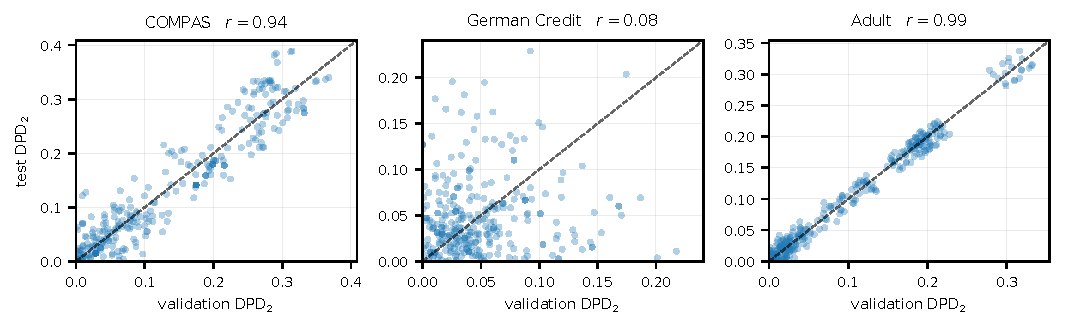
\includegraphics[width=\textwidth]{selection_diagnostic.pdf}
\caption{Validation versus test \dpdtwo{} across sweep configurations. On COMPAS
and Adult the points hug the diagonal --- validation predicts test. On German
they form a cloud.}
\end{figure}

\subsubsection{A second, independent problem: the rule is scale-blind}
The selection rule minimises $\sqrt{(1-\mathrm{acc})^2 + \mathrm{DPD}^2}$. At
German's baseline, $(1-\mathrm{acc}) = 0.270$ but $\mathrm{DPD} = 0.046$, so in
squared terms the accuracy term dominates by \textbf{34.9$\boldsymbol\times$}.
The rule collapses to ``maximise accuracy'' and is nearly blind to fairness ---
even with perfect, noise-free data. On COMPAS ($1.1\times$) and Adult
($0.7\times$) the terms are coincidentally balanced, which is why it works
there.

\begin{example}[The method \emph{does} work on German --- selection just can't find it]
Bypass selection entirely and fix the group-fairness extreme $\beta = 1$:
\begin{center}
\begin{tabular}{@{}lccc@{}}
\toprule
German, LogReg & Test \dpdtwo{} & Accuracy & Seeds improved \\
\midrule
Baseline ($\alpha{=}1$) & $0.046$ & $0.730$ & --- \\
$\alpha{=}0.5,\ \beta{=}1$ & $\mathbf{0.024}$ & $\mathbf{0.729}$ & $8/10$ ($p=0.020$) \\
\midrule
What selection actually picked & $0.047$ & $0.726$ & --- \\
\bottomrule
\end{tabular}
\end{center}
A \textbf{48\% disparity reduction at zero accuracy cost} was available. The
utopia rule walked straight past it --- across ten seeds it picked
$\beta$ values averaging $0.19$, with \emph{three seeds choosing $\beta = 0$}
(no group-fairness weight at all).

\medskip
\textbf{Caution:} $\alpha=0.5$ gives $p=0.020$ but $\alpha=0.75$ gives
$p=0.193$. Do not cherry-pick $\alpha$ --- that would be exactly the test-set
selection avoided everywhere else. Cite the \emph{pre-specified} ablation
contrast instead.
\end{example}

\begin{keybox}[How to frame German in the paper]
Not ``the method fails on German.'' Instead: \emph{the selection procedure fails
on German, and here is the diagnostic proving it.} This is a genuinely useful
methodological finding --- \textbf{validation-based fairness model selection has
a sample-size floor} --- because fairness metrics are differences of
\emph{conditional} rates, so their effective sample size is set by the smallest
group, not by $n$.
\end{keybox}

\subsection{Comparison against established baselines (RQ3)}

\begin{center}
\small
\begin{tabular}{@{}lcc@{\hspace{2.5em}}cc@{}}
\toprule
& \multicolumn{2}{c}{\textbf{COMPAS}} & \multicolumn{2}{c}{\textbf{Adult}} \\
\cmidrule(lr){2-3}\cmidrule(lr){4-5}
\textbf{Method} & Accuracy & \dpdtwo{} & Accuracy & \dpdtwo{} \\
\midrule
Reweighing        & $0.656$ & $\mathbf{0.034}$ & $0.840$ & $0.090$ \\
ExpGrad (DP)      & $0.658$ & $\mathbf{0.035}$ & $0.830$ & $\mathbf{0.013}$ \\
ThresholdOptimizer& $0.663$ & $0.037$ & $0.827$ & $\mathbf{0.009}$ \\
\rowcolor{accentlt} \textbf{Ours (Fair LR)} & $0.661$ & $0.061$ & $0.830$ & $0.021$ \\
\rowcolor{accentlt} \textbf{Ours (Fair MLP)} & $0.669$ & $0.082$ & $0.836$ & $0.026$ \\
XGBoost (no fairness) & $0.655$ & $0.228$ & $\mathbf{0.868}$ & $0.181$ \\
Random Forest         & $0.624$ & $0.164$ & $0.843$ & $0.193$ \\
\bottomrule
\end{tabular}
\end{center}

\begin{warnbox}[Honest verdict: competitive, not superior]
At matched accuracy, the dedicated group-fairness methods reach modestly lower
DPD than the composite loss. \textbf{Do not oversell this --- and you don't need
to.} Your contribution is the trade-off map, not a new state of the art.

The correct framing: \emph{``the composite loss achieves group-fairness levels
comparable to established methods, which establishes it as a credible
instrument for probing the trade-off --- and unlike those methods, it exposes a
continuous, controllable interpolation between the two fairness notions.''}
None of ExpGrad, ThresholdOptimizer, or Reweighing has a $\beta$-equivalent.
That is your differentiator.
\end{warnbox}

One more useful observation: \textbf{XGBoost on Adult} has the highest accuracy
($0.868$) \emph{and} one of the largest disparities ($0.181$). The most accurate
model is among the least fair --- a clean one-sentence motivation for the whole
paper.

\begin{figure}[htbp]
\centering
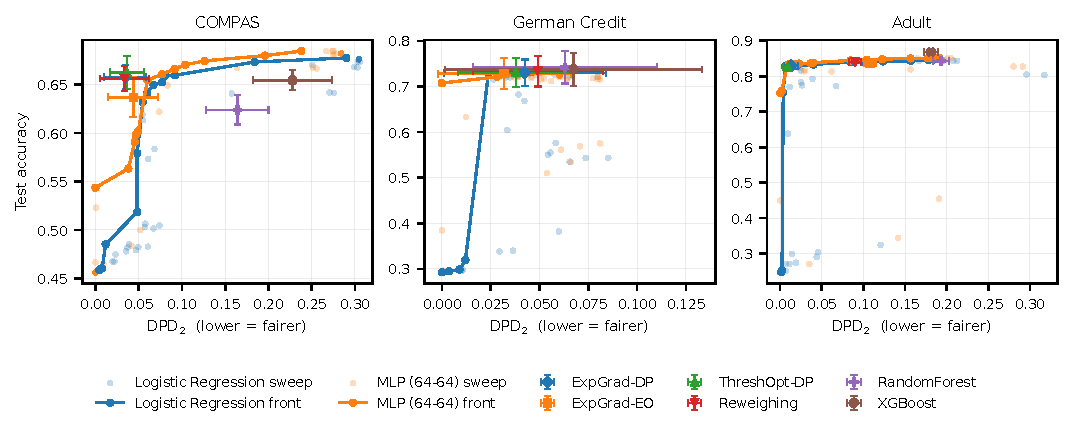
\includegraphics[width=\textwidth]{pareto_frontiers.pdf}
\caption{Accuracy versus \dpdtwo{}. Faint points are sweep configurations, solid
lines the Pareto fronts, markers the baselines with error bars.}
\end{figure}

\subsection{What can we reasonably conclude?}

\begin{center}
\small
\begin{tabular}{@{}p{0.47\textwidth}p{0.47\textwidth}@{}}
\toprule
\textcolor{good}{\textbf{Supported by our data}} &
\textcolor{warn}{\textbf{NOT supported --- do not claim}} \\
\midrule
A group-fairness objective produces large, significant reductions in group
metrics (up to $-89\%$ DPD) at $\approx1.5$ accuracy points, where a disparity
exists. &
That our method beats established baselines. It doesn't; it matches them. \\
\addlinespace
That improvement carries a \emph{measured} cost to individual fairness
($+5$--$14\%$ GE) and, on Adult, a severe cost to equalized odds
($2.3$--$3.3\times$). &
Anything about individual fairness in the Dwork ``similar individuals'' sense
--- GE(2) is an inequality-of-outcomes measure. \\
\addlinespace
An individual-fairness objective improves individual fairness weakly and group
fairness not at all. &
Any COMPAS EOD conclusion --- that column is noise-dominated by 11-person
groups. \\
\addlinespace
The pattern holds across two architectures and two of three datasets; the third
is explained, not contradictory. &
Any conclusion resting on the Gini column --- it is $1-$selection rate. \\
\addlinespace
The composite loss reaches group-fairness levels comparable to
Reweighing / ExpGrad / ThresholdOptimizer. &
Generalisation beyond tabular binary classification with a single sensitive
attribute. \\
\bottomrule
\end{tabular}
\end{center}

\clearpage

%%%%%%%%%%%%%%%%%%%%%%%%%%%%%%%%%%%%%%%%%%%%%%%%%%%%%% 7. PAPER PREPARATION
\section{Research Paper Preparation}

What belongs in each section, based on the methodology and results above.

\subsection{Introduction}
\begin{itemize}
\item Open with concrete stakes: COMPAS, credit, hiring. One sentence, no
melodrama.
\item Establish that ``fairness'' is not one thing --- group vs individual, with
a one-line intuition for each.
\item State the gap: impossibility results tell us the definitions conflict
\emph{in principle}; far less work measures \emph{how much}, with error bars,
across datasets.
\item State the contribution list explicitly (reviewers look for this):
(1) a differentiable composite loss with a single interpolation parameter;
(2) an empirical trade-off map over 2{,}940 models;
(3) significance-tested comparison against all three mitigation families;
(4) a documented label-leakage correction to a COMPAS feature set.
\item Preview the headline: $-89\%$ DPD on Adult at $-1.5$ accuracy points,
with EOD $2.6\times$ worse.
\end{itemize}

\subsection{Related Work / Literature Review}
Four blocks:
\begin{enumerate}
\item \textbf{Group fairness definitions \& methods} --- demographic parity,
equalized odds (Hardt et al.\ 2016), Reweighing (Kamiran \& Calders 2012),
ExponentiatedGradient (Agarwal et al.\ 2018). Cite what you actually ran.
\item \textbf{Individual fairness} --- Dwork et al.\ (2012) Lipschitz
formulation; Speicher et al.\ (2018) benefit-vector formulation. \textbf{Be
explicit that you use the Speicher operationalisation, not the Dwork one}, and
say why (computable without a similarity metric).
\item \textbf{Impossibility \& tension results} --- Kleinberg et al.\ (2016);
Chouldechova (2017); Barocas, Hardt \& Narayanan. This is the theory your Adult
result empirically confirms.
\item \textbf{COMPAS as a benchmark and its critiques} --- ProPublica's
analysis, the rebuttals, and the feature-set/leakage literature. This is where
your \code{duration} fix lives.
\end{enumerate}
Position the gap in one sentence: prior work either proves conflict
theoretically or optimises one notion at a time; you \emph{interpolate
continuously} and measure both.

\subsection{Methodology}
\begin{itemize}
\item The loss equation, with SoftDP and SoftGE derived and the benefit vector
explained.
\item \textbf{Why surrogates are necessary} --- the thresholding step function
has no gradient. Make this the motivating argument.
\item Architectures, optimiser, full-batch training, early stopping.
\item The validation-only utopia-distance selection rule and the $5\%$/$95\%$
degeneracy guard, both with justification.
\item \textbf{Do not put results here.}
\end{itemize}

\subsection{Experimental Setup}
\begin{itemize}
\item Dataset table: $n$, target, sensitive attribute, group sizes, per-group
base rate, encoded dimensionality.
\item Preprocessing: $60/20/20$ per seed, scaler + one-hot, fit on train only.
Note splits are unstratified.
\item The COMPAS filter list and the \code{duration} removal with its $-0.78$
correlation and mechanical explanation. Frame the accuracy drop as correctness.
\item Grid: $\alpha,\beta$ value lists; total model count.
\item Ten seeds control split $+$ init $+$ stochastic baselines.
\item Baseline configurations with hyperparameters.
\item Metric definitions \textbf{with the corrected GE(2) naming}, and the
largest-2-groups DPD with its tiny-group justification (quote the Asian $n=31$ /
Native American $n=11$ numbers --- they make the argument for you).
\item Statistical protocol, and note that $p = 1/512$ is the floor at $n=10$.
\item Reproducibility: library versions, CPU-only, checkpoint caching, exact
commands.
\end{itemize}

\subsection{Results}
Order by strength, not by figure number:
\begin{enumerate}
\item \textbf{The $\beta$ cross-effect and ablation.} Lead with this; it is the
contribution.
\item \textbf{Fair vs baseline with significance.} COMPAS and Adult positive,
German null.
\item \textbf{Adult's DPD/EOD inversion} --- its own subsection, with the base
rate numbers. Your theory-confirmation result.
\item \textbf{Pareto frontiers with baselines overlaid} (RQ3).
\item \textbf{German null result} --- its own short subsection with the
selection diagnostic. Reporting it plainly is a credibility asset.
\item \textbf{Supplementary} --- surrogate validation, seed-mean heatmaps.
\end{enumerate}
Every number as mean $\pm$ std over ten seeds. Every figure with error bars.

\subsection{Discussion}
\begin{itemize}
\item Interpret the \textbf{asymmetry}: why the group objective works strongly
and the individual objective weakly (freely controllable quantity vs a floor set
by irreducible error).
\item Interpret the \textbf{Adult inversion} as the empirical face of the
impossibility theorem, with the exchange rate quantified.
\item \textbf{What $\beta$ means for a practitioner}: not a hyperparameter to
tune for performance, but a \emph{policy dial} encoding which fairness notion the
institution has committed to. This is the most quotable idea in the paper.
\item \textbf{Why German shows nothing}, and what it implies about model
selection at small $n$.
\item Position vs baselines honestly.
\item The uncomfortable normative point: Adult MLP at $\beta=1$ gives DPD
$0.009$ --- near-perfect demographic parity --- while making error rates markedly
\emph{more} unequal. Fairer by one definition, less fair by another. Don't
resolve it; that tension is the paper.
\end{itemize}

\subsection{Limitations}
Be thorough --- it buys credibility, and every item is real and verifiable:
\begin{enumerate}[itemsep=1pt]
\item GE(2) is not Dwork-style individual fairness.
\item Gini as implemented equals $1-$selection rate.
\item COMPAS EOD (and all-groups DPD) dominated by groups of 11--31 people.
\item German Credit underpowered at $n=1000$; selection unstable.
\item Full-batch training, one gradient step per epoch, max 300 steps.
\item Single binary/categorical sensitive attribute; no intersectional analysis.
\item Fixed $0.5$ threshold, unlike ThresholdOptimizer.
\item Utopia-distance selection implicitly weights 1 accuracy point $=$ 1 DPD
point, and is scale-sensitive.
\item Sensitive attribute included as a model input.
\item Adversarial debiasing not run.
\item Positive-class polarity inconsistent across datasets.
\item Tabular binary classification only.
\item Splits are unstratified.
\end{enumerate}

\subsection{Conclusion}
Restate compactly: a differentiable composite loss lets $\beta$ interpolate
continuously between group and individual fairness; sweeping it across three
datasets, two architectures and ten seeds produces an empirical map showing the
group objective strongly reduces group disparity ($-78\%$ to $-89\%$ DPD) at a
small accuracy cost ($\approx1.5$ points) and a measurable cost to individual
fairness and equalized odds; the individual objective helps individual fairness
only weakly and group fairness not at all; the effect vanishes where the
baseline is already near parity. Close on the practitioner-facing point:
\textbf{$\beta$ is a policy parameter, not a tuning knob} --- the trade-off
cannot be engineered away, only chosen.

\subsection{Before you write: five fixes, ranked}

\begin{center}
\small
\renewcommand{\arraystretch}{1.2}
\begin{tabular}{@{}c p{0.27\textwidth} p{0.40\textwidth} p{0.11\textwidth}@{}}
\toprule
\textbf{\#} & \textbf{Issue} & \textbf{Why it matters} & \textbf{Effort} \\
\midrule
1 & Relabel ``Theil Index'' $\to$ \textbf{GE($\alpha{=}2$)} &
Currently mislabelled against the standard definition; a knowledgeable reviewer
will catch it. No numbers change. & Text only \\
2 & Drop or relabel the Gini column &
It is exactly $1-$selection rate; presenting it as individual fairness is not
defensible. & Text only \\
3 & Add largest-2-groups EOD for COMPAS, or caveat it &
COMPAS EOD is currently pinned by groups of 11 and 31 people. & $\approx$10
lines $+$ rerun \\
4 & State explicitly: sensitive attribute is an input; training is full-batch;
splits unstratified &
All three are choices reviewers will ask about. & Text only \\
5 & Frame German as a \emph{reported null result} with its diagnostic &
Reporting it plainly is a credibility asset and it supports RQ2. & Text only \\
\bottomrule
\end{tabular}
\end{center}

\begin{keybox}[Status]
Fixes 1, 2, 4 and 5 have already been applied in the IEEE paper produced
alongside this guide. Fix 3 is documented there as a stated limitation with the
remedy named.
\end{keybox}

\vspace{1.2cm}
\begin{center}
\rule{0.5\textwidth}{0.4pt}\\[6pt]
\small\textit{End of study guide.}
\end{center}


\end{document}
